%defining document class
\documentclass{article}
\usepackage[utf8]{inputenc}
%setting up page layout
\usepackage{lipsum}
\usepackage[margin=1in,left=1.1in,includefoot]{geometry}
%Inserting package to import picture/images
\usepackage{graphicx}
% allows control of float positions
\usepackage{float}
%start compiling document
\begin{document}
% creating title page
\begin{titlepage}
%defining alingment of content
	\begin{center}
    \line(1,0){475}\\
% defining spacing    
   [2.5mm]
    \huge{\bfseries DATA SCIENCE TEAM REPORT}\\
    \line(1,0){475}\\
    [3mm]
    \textsc{\Large Using Data Analytics For Business}\\
    [6cm]
    \textsc{\small Product Proposal for Data Science\\
    [1mm]
    Data Engineering Studio A\\
    \line(1,0){150}\\
    Spring 2017}\\
    [7cm]
    \end{center}
% shifting alingment to left    
    \begin{flushleft}
% inserting line    
    \line(1,0){500}\\
    \textsc{\large Name: Sudip Siwakoti\\
     Student Number: 12956936\\
     Email: sudip.siwakoti@student.uts.edu.au}\\
    \end{flushleft}
    \lipsum[0]
\end{titlepage}
%inserting table of content.
\tableofcontents
% removing page number form table of content
\thispagestyle{empty}
%clearing rest of the page
\cleardoublepage
%resetting page number 
\setcounter{page}{1}
%starting section and labeling section
\section{Introduction}\label{sec:intor}
	As human race has been collecting data and using it to improve almost since the beginning of time. If we go through the history of mankind we can see that formally or informally we have been collecting data and analyzing it to make things better and gain understanding and knowledge from the observation. In past decayed or so we have change the way and how we collect and analyze the data and created field of study that is dedicated on finding scientific methods to explore and visualize data, this field of study is known as data science. Data science is a "concept to unify statistics, data analysis and their related methods" in order to "understand and analyze actual phenomena" with data. With the increase in computing power of modern computers and the way we collect data, Data Science can help us understand every aspect of our life better.\\\\
The project that I have taken on my Data Studio A is a Data science project for a retail insurance company. For this project I have been provided with a set of data from the insurance company’s database. I performed different analysis based on the knowledge and skill that I learned overtime during Studio A session. Using these skills set I have prepared an analytical report which can provide a bit of insight into the data using Excel and Power BI. During the entire period of this project I acquired knowledge on using Power Query and Power Pivot, Power BI and Tableau and based on the knowledge and skills that I have learned I will be bringing forward about the advantage and disadvantages of each platform and which platform will better suit the client.\hfill \pagebreak
%starting new section
\section{DATA MINING CONCEPTS}\label{SEC:background}
Data mining is the process of extracting meaningful information from large sets of data using mathematical and statistical analysis to visualize existing trend and pattern within the data. These pattern and trends within the data can be then used to create a data model which can be used to predict/forecasting, Risk analysis and calculating probability, recommendation on particular subject, etc. Creating a data mining model is a part of larger process brainstorming, model creation, implementation, evaluation, etc. Following steps can be used to define the process and also can be represented by the diagram below:\\

%importing figure and defining location
\begin{figure}[h!]
	\centering
    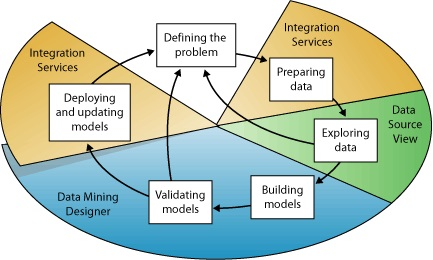
\includegraphics[height= 8cm,width=0.8\textwidth]{data-mining-process.jpg}
    \caption[optional caption]{Data Mining Process}
    \label{fig:Data Mining Process}
\end{figure}

\subsection{Defining the Problem}\label{concept}

Defining the problem clearly is first step to data mining. To define the problem one needs to understand the problem and when you understand you can utilize the data set to create different ways to answer the underlying problem. At this stage, one needs to analyses client requirements and scope of the problem, defining evaluation methods and objective of the model. Some examples are what is one looking for in the dataset and what are the relationship we are trying to find within the data? What is the objective of the model and what does client wants?

\subsection{Preparing Data}\label{concept}	

This step in the data mining is to clean and consolidate the data from above step one. This is one of the important step in data mining process as data can be scattered within the client’s business and also can be in different formats, filled with inconsistencies, missing or corrupted data within the dataset. Some examples of these kinds of data are wrong or unrelated information such as blank cell where there should be name of state or a state that is not even in the related country. Preparation and cleaning of data is not just about removing bad or missing data but is an opportunity to study the data and find correlation within the data, mind mapping of data and determining appropriate methods of analysis. During this process you can also get what might be the limitations of  data and prepare yourself for ways to overcome the limitations. In a very large datasets as one used for data mining it is not possible for analysis to go through each an every rows and columns of data so some form of automated data cleaning and filtering should be used.

\subsection{Exploring Data}\label{concept}

Third step in data mining is Exploring data which is like building relationship with data to understand and learn about the dataset. Without understanding the data you won’t be able to  make appropriate decision and create a well defined data mining model. You can use different calculating technique such as minimum values, maximum values, mean, standard deviation, etc. Exploring data through these techniques you can give you better understanding the level of accuracy of the given datasets and what might be the solution to resolve any inaccuracy or what kind of result to expect.

\subsection{Building Model}\label{concept}

In this step we use the knowledge and insight gained during data exploration to create a data model. Selected columns of data is used to create a mining structure which is then linked to the source data. Mining structure is like a empty container which defines certain attributes of the model to process data but does not itself contain any data. Data model can use and adjust parameters as per algorithm’s needs and can apply filters to train data to use just a subset of the data.

\subsection{Exploring and Validating Models}\label{concept}

In this step of data mining the analyst tests the data using different models created in step 4 to yield results. The results are then compared with the problem definition to find the best solution for the problem. Also the model is tested for accuracy of the model by creating prediction queries which can be done automatically while building the mining model. Once a valid data model is identified it is then passed on to next step while if the results are not as required or expected then the it is passed back to modeling team where the modeling team once again build other possible models for exploring and validation of models.

\subsection{Deploying and Updating Model}\label{concept}

The last step in data mining process is deployment and updating of models. Once the mining model is implemented in production environment, implemented model will be able to make predication and forecasts for the customer where these predications/forecasts will be used to make decision. Using the implemented models one can create reports that lets users directly query against an existing mining model.\\\\
As the more data is acquired with time the existing mining model needs to be updated to increase the accuracy of the model. Also with creation of data model the modeling team can make suggestion for improvement of data collection methods and processed to increase the productivity and effectiveness of the model. Based on the new and improved models from new data, implemented models are updated.\\\\
Through data mining clients can not only be able to get results and reports from the data but can also make changes and updates to the data collection methods to make it more efficient and effective which in return make the data models more powerful and accurate. Within data mining there are few terms and concepts that a data analyst team should understand and are explained below.(Microsoft 2017)\pagebreak

\section{DATA CLASSIFICATION AND PREDICTION}\label{classification}

There are two forms of data analysis that can be used to extract models which describes classes or predicts future data trends and they are
\begin{itemize}
\item Classification
\item Prediction
\end{itemize}


\subsection{What Is Classification?}\label{classification}
Classification is a method of categorically labeling a class of data to perform an analysis. For example, 
If a bank want to know which of its customer(credit applicant ) based on level of risk associated with lending then they can classify their customers based on their risk category (low, medium, High). While doing this classification all the customers from this data would be categorically separated into fixed category mentioned above ie model or classifier is constructed to predict the categorical labels.

\subsection{What Is Prediction?}\label{classification}

Prediction is a method of statistical analysis used in data mining to predict future trend or pattern based on past statics. For example, An electronic manufacturing company wants to predict sales of its new product being launched based on its past product launch statistics to estimate production of its new product.

Another example is a store want to predict how much a given customer will spend during a sales on Boxing day. Based on this prediction the store can set a performance target and also make stock ordering to achieve the target.



\section{DATA CLUSTERING }\label{sec:analysis}
Data clustering is defined as method/process of grouping or organizing abstract object into classes of similar object. During data clustering dataset is first partitioned into groups based on their similarities and labeled. The main advantage of  data clustering over classification is it is adaptable to changes and can help single out useful features that distinguish different groups. Some of the application of cluster analysis are listed below.
\begin{itemize}

\item Clustering analysis is mainly used in market research, pattern recognition, data analysis and image processing applications.
\item	Using clustering marketers can discover distinct groups of customer base and characterize the group based on their purchasing patterns.
\item	It can also be used in  genetics to categories genes with similar function and gain insight into structures inherent to populations.
\item It can also be used in outliers detection application such as credit card fraud detection.
\item	Clustering also gives insight into the distribution of data in data mining process.
\end{itemize}\pagebreak

\subsection{Clustering Methods }\label{sec:data clustering methods}

Clustering methods are mainly categories on following types
\begin{itemize}
\item Partitioning method
\item Hierarchical method
\item Density-based method
\item Grid-Based Method
\item Model-Based Method
\item Constraint-based Method
\end{itemize}

\subsubsection{Partitioning Method}\label{clustering methods}
In this method a database of ‘n’ object and the partitioning method construct of ‘k’ partitions of data then each partition will represent a cluster and k=<n. It means that it will classify the data into k groups, which satisfy following requirements:
\begin{itemize}
\item Each group contains at least one object.
\item Each object must belong to exactly one group.
\end{itemize}
Also for a given number of partition ‘k’ , the partitioning method will create an initial partitioning and then it uses the iterative relocation of technique to improve the partitioning by moving objects from one group to other.

\subsubsection{Hierarchical method}\label{clustering methods}

This method creates a hierarchical decomposition of the given set of data objects. We can classify hierarchical methods on the basis of how the hierarchical decomposition is formed. There are two approaches
\begin{itemize}
\item Agglomerative Approach\\
This approach is also known as the bottom-up approach. In this, we start with each object forming a separate group. It keeps on merging the objects or groups that are close to one another. It keep on doing so until all of the groups are merged into one or until the termination condition holds.\\

\item Divisive Approach\\
This approach is also known as the top-down approach. In this, we start with all of the objects in the same cluster. In the continuous iteration, a cluster is split up into smaller clusters. It is down until each object in one cluster or the termination condition holds. This method is rigid, i.e., once a merging or splitting is done, it can never be undone.
\end{itemize}

\subsubsection{Density-based method}\label{clustering methods}
This method is based on the notion of density. The basic idea is to continue growing the given cluster as long as the density in the neighborhood exceeds some threshold, i.e., for each data point within a given cluster, the radius of a given cluster has to contain at least a minimum number of points.\pagebreak

\subsubsection{Grid-Based Method}\label{clustering methods}
In this, the objects together form a grid. The object space is quantized into finite number of cells that form a grid structure.
\subsubsection*{Advantage}\label{Grid-Based Method}
\begin{itemize}
\item The major advantage of this method is fast processing time.
\item is dependent only on the number of cells in each dimension in the quantized space.
\end{itemize}

\subsubsection{Model-Based Method}\label{clustering methods}

In this method, a model is hypothesized for each cluster to find the best fit of data for a given model. This method locates the clusters by clustering the density function. It reflects spatial distribution of the data points.
This method also provides a way to automatically determine the number of clusters based on standard statistics, taking outliers or noise into account. It therefore yields robust clustering methods.

\subsubsection{Constraint-based Method}\label{clustering methods}

In this method, the clustering is performed by the incorporation of user or application-oriented constraints. A constraint refers to the user expectation or the properties of desired clustering results. Constraints provide us with an interactive way of communication with the clustering process. Constraints can be specified by the user or the application requirement.



\section{SCOPE OF PRODUCT AND INTEGRATION}\label{sec:Scope}
In this project the scope of product the has been developed is to analyze the given datasets to create a model to prepare a report and make a recommendation on best suited platform from a preselected set of analytics platforms. Also make recommendation on any update on data collections methods that can be more productive and efficient to create a better data model.  The report created from the database must be able to give a general overview of market and consumer, existing trend within the dataset, etc. The final report will be presented to the product owner which can be used to analyze future data collection and reporting. Data cleaning and basic level filtering of data has been automated and implemented within the report creating platform and future report can be created dynamically as required by the product owners. 

\section{WORKPLACE ENVIRONMENT AND SCHEDULE CONSTRAINTS}\label{sec:constrains}
During the project, I faced few workplace environment and schedule constrains which is normally not present in a real-life work environment. The major workplace environment constrains was not having data on time and direct access to data, lack of understanding of data collection methods and lack of problem definition from product owners. Also, lack of human resource within the team created unnecessary strain and workload on product development team. Lack of human resources directly impacted on the level of research that could be conducted on given time frame and limited the sharing of knowledge and ideas within the team which is a key ingredient of a productive work environment. Another key aspect is schedule constraints as a student I had limited time that I could spend on the product development and data exploration. Having ample time for data exploration can provide excellent insight into data mining and modeling which in return can create better and accurate data model for the business giving better insight into the available data. Not having access to data on time created an additional time constrain as I had to other commitments for other subjects through the semester.(Tutorial Point 2017)

\section{DESIGN PROCESS}\label{sec:Design}

Data mining includes different steps that the product development needs to go through and the steps
\subsection{Problem Definition}\label{Defination}
Problem definition for the product was to analyses using appropriate data model and suggest an appropriate platform/software for data visualization and make any recommendation for future update.
\subsection{Preparing And Exploring Data}\label{cleaning}
Data was cleaned using Power Query editor in Excel. Power query editor is also available in Power BI so any interface can be used for data cleaning. During the cleaning selected column of data were selected as per preselected possible models and applied Grouping function within Query editor and different filters were applied to the data to further clean the data. Once cleaning of data was finished and finalized the process of cleaning was automated by using manage parameter function and invoking a custom function in power query. Manage parameter function sets a predefined path and filename where as query with invoke function creates a template for future data to be cleaned and brought within the model with limited manual input. Data is  and possible new data model were noted during this process.
\subsection{Building Model And Validating}\label{building}
Based on exploration all possible model were built using the custom column selected during the  preparation process. All the models that were created were then tested against the problem definition and tested for accuracy. For this process Power BI was used as it has easy to use built in data visualization options. Different visualization was created and most suitable and accurate visualization was selected to prepare the report
\subsection{Deploying And Updating Model}\label{deploying}
For this stage of the project, the final report will be presented to the product owners and a consultation session will be held. In the session, the report and its usage will be demonstrated and also the limitations will be explained. Further to the process, updating model will be done in consultation with the product owners. Current data has some limitations on what can be done and also current data collection has extensive missing data and inappropriate formatting which has led to inaccurate data model. The data can be made more accurate changing few parameter in data collection methods like data recorded date on the data will be helpful to create a prediction model for future business performance. Accurate data record date will add the ability to do an analysis at any given time. Also using R script in Power BI can be helpful and productive as R is more powerful than Power BI and running a R script in Power BI will make data model more accurate and effective. You can also use R script to run different algorithm for data clustering and visualization which will give more dynamics to the data model. Future, data model will include a custom written R script running in the background of Power BI for in-depth analysis of data. Also future model will incorporate data sets from Google Analytics additional visualization of data.\pagebreak

\section{ADVANTAGES AND LIMITATION OF SELECTED SOFTWARE OPTIONS }\label{sec:SOFTWARE OPTIONS}
During the development phase Power BI, Power Query, Power Pivot and Tableau were considered as Power BI incorporates Power query and Power Pivot within itself it is best to compare Power BI and Tableau head on. Both of the software’s has their limitation and advantages while I have noted few differences while perusing the project. 
\subsection{Advantages of Power BI }\label{advantages}
\begin{itemize}
\item Incorporates many known features from excel and it data analytics tool.
\item Familiar UI for excel users.
\item Easy to run R scripts and algorithms.
\item Easy report Sharing within an organizational environment. 
\item Powerful processing and visualization engine.
\item Big community forum for help with different problems.
\item Ability to view data dynamically in reports.
\end{itemize}

\subsection{Limitation of Power BI }\label{Limitation}
\begin{itemize}
\item Limited pre-built data visualization options.
\item Does not fully support geo-location visualization for Australia
\item Unfriendly and tedious user interface for first time user.
\end{itemize}
\subsection{Advantages of Tableau }\label{advantages}
\begin{itemize}
\item Full support for geo-location visualization for Australia.
\item User friendly UI.
\item Easy report sharing within an organizational environment. 
\item Easy to use analytics tool.
\end{itemize}
\subsection{Limitation of Tableau }\label{Limitation}
\begin{itemize}
\item Hard to incorporate R script.
\item Limited pre-built data visualization options
\item Need to learn the software from basics
\end{itemize}
\section{LIMITATIONS OF IMPLEMENTED MODEL }\label{sec:Limitation of model}
Currently developed data model does not incorporate all possible data models and has limitation. Presented model cannot make predication at this point in time. Also the data model’s accuracy has not been tested to the full extension and hence accuracy cannot be predicted. The model also lacks ability to visualize differences between datasets of two different period currently. There also exist some bugs within the model currently creating different set of column when comparison between two different weeks of data which cannot be seen when drilling through the dataset but only occurs in visualization which directly impacts the data Visualization abilities of the model. \\

This analytics model was created using Power BI assuming that currently BWM uses Excel data analytics features for their data analysis and to minimize the impact on organizational level that would be created due to transitioning between different platform but Tableau is also a good platform to that can maximize good results in data analytics.\pagebreak

\section{REFLECTION}\label{sec:Reflection}


Data studio A started with lots of excitement as we had a bit of insight into the subject from our earlier session during Autumn session of introduction to data engineering that studio will be about developing a product based on real life work environment on data analytics. On the first week of studio we participated in brief introduction on products available for development. After brief introduction into the subject were asked to describe about the products we were introduced to our fellow students and we marked each other on a survey based on description we provided to the fellow students. Also during this first session we expressed our interest on a subject/product and separated the group. There were lot of students interested in Data Science product but there was only one product owner in the beginning more products were introduced. With the introduction of new product 3 teams were constructed by our subject coordinator. On my group we had 3 members including myself. My team was assigned with a product, which was to create a data analytic tool/report for BWM. BWM is an insurance company that resells insurance products for pets which they acquired from a wholesaler.\\ 

On second week of the session one of the member of my team withdrew for the subject and was left with two member. On this week we were also introduced to different methods and applications used in the industry like overleaf/Latex application for report creation, Version control application to track and be in control of changes in made during the product development life cycle, Trello dashboard to track team performance, etc.\\

During this period we also decided on application and environment we will be using to create the data model for the dataset that would be provided to us and we selected R programming language as preferred application as a product development software. With the selection of product development application we started learning on how to use R for data mining and modeling. Meanwhile, during this time another member of my team withdrew for the subject and I was by myself for the whole project. Still after all the changes within my team I decided to continue with the project on my own still being aware that it will be a lot of work for myself to complete the project. I started learning and acquiring knowledge on data science, data mining methods and modeling and the selected platform by watching tutorial on Lynda.com, youtube, and researching into different articles, papers on data science and R documentation.\\

Meanwhile, I was given a topic to research on Google Analytics for a presentation as I was also planning to prepare a report for the product owner based on their website using google analytics. I learned about google analytics and how it can be used to generate report for business decision making and understanding customer behavior. I also learned google analytics research that the dataset acquired from google analytics could be used to create a better model for the product owners. It was nearly week 7 into the session and I still had not got dataset for the product owners to work on the dataset. This prospect of not having data till this late into the session had started to bother me and also made me nervous that I would not be able to finish my project on time.\\

On the 8th week I received data from my product owner and with a surprise all the plans and structure of the project was changed. Now it was decided that I would be using excel, Power pivot, power query and Power BI to make certain prediction and create a report and recommendation based on the provided dataset. I was somewhat familiar with excel but I had never used Power Query, Power Pivot and Power Bi so I had to start all over again to learn use these platform. This significantly consumed my schedule and as I was approaching end of spring session I had commitments to other subjects I had very little time to get on with the project. From Robin’s recommendation I had attend a workshop on Tableau a data analytics software earlier in the session and had gained some insight into its usages. While learning new data analytics platforms used in the industry I also started cleaning and exploring the data provided and mind mapping possible data models. The provided raw data had lot of missing, incorrect and unusable data which eventually created headache and frustration for me and constrained my little available time.\\

Data from Tipping point (Company used by BWM to collect their web data) was almost useless as it had lot of missing data and could not be used for analytics and modeling. The only data I had was the weekly policy information collected by the company. Even this data had around 15-20 percentage of missing or incorrect data. After cleaning data and selecting particular columns for data modeling using Power Query editor I created a model and used Pivot Table and chart in excel to create report but due to limited knowledge and time constrain I struggled a lot create a report using Pivot Tables and charts on excel. On top of this there was lot of software limitation that would directly impact on performance of data modeling. Pivot tables on 32 bit version of excel had memory and processing limitation and 64 bit version had its own drawbacks. Excel itself is not much powerful data analytics tool as it is slower take lot of processing time and there is limitation on dynamics of the software as what can be done as well. As PowerBi is specifically designed for data analytics and is almost similar to excel and power pivot and query. It also facilitates a dashboard to create reports from a database and share the reports within an organization easily. The reports created can be viewed dynamically in Power BI but it has its limitations as well, specifically when creating report there are set no of visualization available and it is hard to combine multiple data within a graph apart from 2 available visualization options. One of the major benefit of PowerBi is the ability to use custom R script for visualization and data modeling as features of R is embedded within the software. Due to the changes during the session I could not completely learn R and could not complete later due to time constrain. Only if I had data earlier in the session then I could have created better model using R script in PowerBI to make data more dynamic.\\

By the end of this semester of Data Studio A I have understood the need of team member to share task in a project like this one and how sharing knowledge within the team member could be helpful and productive by significantly reducing pressure within the team. Also, I have decided to continue with the product in Studio B to further develop a better model for the product owner. Studio A has also provided me insight into the industry and its environments and the challenges within the industry. I also provided me with enlightenment on to the pathway to better data analytics skills.\pagebreak

\section{REFRENCES}\label{refrences}

Microsoft 2017, Data Mining Concepts, Organisation, Microsoft, US, viewed 10/25 2017, <https://docs.microsoft.com/en-us/sql/analysis-services/data-mining/data-mining-concepts>.\linebreak\linebreak
TutorialsPoint 2017, Data Mining, Educational website, Tutorials Point Simply Easy Learning, India, viewed 10/25 2017, $<https://www.tutorialspoint.com/data_mining/dm_cluster_analysis.htm>.$
\end{document}